\section{Comparison of the classical cross-entropy and the \UncertaintyLoss}
\label{uncertain_loss_classification}

\subsection{Simple classification task}

In this section, we do not consider temporal data. The goal of this experiment is to show the benefit of the \UncertaintyLoss compare with the classical cross-entropy loss on a simple classification task. As a consequence, we do not consider RNN in this section. We use a simple two layers neural network to predict the concentration parameters of a Dirichlet distribution from the input vector.

\textit{Set-up.} The set-up is similar to \cite{PriorNetworks} and consists of two datasets of 1500 instances divided in three equidistant 2-D Gaussians. One dataset contains non-overlapping classes (\textbf{NOG}) whereas the other contains overlapping classes (\textbf{OG}). Given one input $x_i$, we train simple two layers neural networks to predict the concentration parameters of a Dirichlet distribution $\textbf{Dir}(\alpha_1(x_i), \alpha_2(x_i), \alpha_3(x_i))$ which model the uncertainty on the categorical distribution $\bm{p}(x_i)$. On each dataset, we train two neural networks. One neural network is trained with the classic cross-entropy loss $\mathcal{L}^{\text{CE}}$ which uses only the mean prediction $\bar{\bm{p}}(x_i)$. The second neural network is trained with the \UncertaintyLoss loss plus a simple $\alpha$-regularizer:
\begin{equation}
\begin{aligned}
\mathcal{L}^{\text{UCE}} + \bigl\lvert\alpha_0(x_i) - \sum_j  \mathbb{1}_{x_j \in N_w(x_i) }\bigr\rvert
\end{aligned}
\end{equation}
where $x_i$ is the input 2-D vector and $N_w(x_i) = \{x', ||x' - x_i||_2^2 < w\}$ is its euclidean neighbourhood of size $w$. We set $w=10^{-5}$ for the non-overlapping Gaussians and $w=10^{-2}$ for the overlapping Gaussians.

\textit{Results.} The categorical entropy $-\sum_\IndexClass p_\IndexClass(x_i) \log p_\IndexClass(x_i)$ is a good indicator to know how certain is the categorical distribution $\bm{p}(x_i)$ at point $x_i$. A high entropy meaning that the categorical distribution is uncertain. For non overlapping Gaussians (Fig.\ \ref{classic-narrow-cat_entropy} and \ref{new-narrow-cat_entropy}), we remark that both losses learn uncertain categorical distribution only on thin borders. However, for overlapping Gaussians (See Fig.\ \ref{classic-spread-cat_entropy} and \ref{new-spread-cat_entropy}),the \UncertaintyLoss loss learns more uncertain categorical distributions because of the thicker borders.

Other interesting results are the concentration parameters learned by the two models (Fig. \ref{fig:alpha_classification}, Fig. \ref{fig:alpha_classification2}). The classic cross-entropy loss learns very high value for $\alpha_1(x_i), \alpha_2(x_i), \alpha_3(x_i)$ which does match with the true distribution of the data. In contrast, the \UncertaintyLoss learn meaningful alpha values for both datasets (delimiting the in-distribution areas for $\alpha_0$ and centred around the classes for the others).

\begin{figure}[H]
\centering
    \begin{subfigure}{0.245\textwidth}
        \centering
        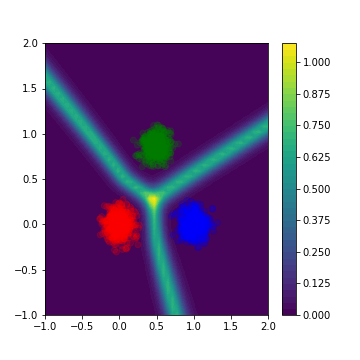
\includegraphics[width=\linewidth]{sections/010_neurips2019/paper/images/classic-narrow-cat_entropy.png}
        \caption{NOG - CE - Cat. Ent.}
        \label{classic-narrow-cat_entropy}
    \end{subfigure}
    \begin{subfigure}{0.245\textwidth}
        \centering
        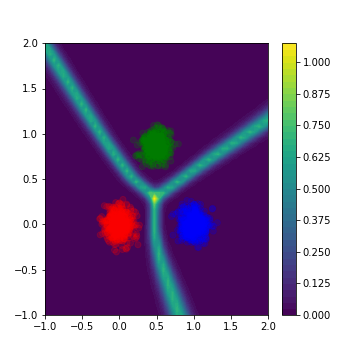
\includegraphics[width=\linewidth]{sections/010_neurips2019/paper/images/new-narrow-cat_entropy.png}
        \caption{NOG - UCE - Cat. Ent.}
        \label{new-narrow-cat_entropy}
    \end{subfigure}
    \begin{subfigure}{0.245\textwidth}
        \centering
        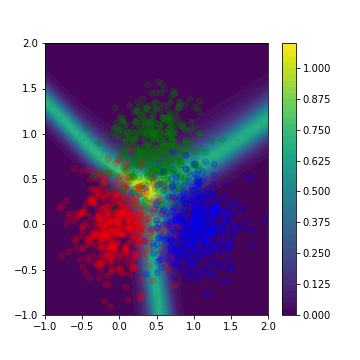
\includegraphics[width=\linewidth]{sections/010_neurips2019/paper/images/classic-spread-cat_entropy.png}
        \caption{OG - CE - Cat. Ent.}
        \label{classic-spread-cat_entropy}
    \end{subfigure}
    \begin{subfigure}{0.245\textwidth}
        \centering
        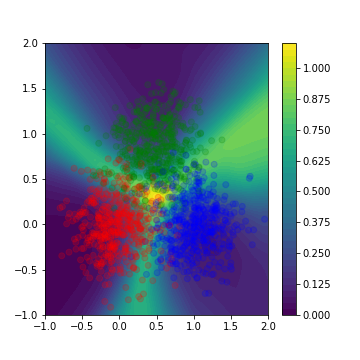
\includegraphics[width=\linewidth]{sections/010_neurips2019/paper/images/new-spread-cat_entropy.png}
        \caption{OG - UCE - Cat. Ent.}
        \label{new-spread-cat_entropy}
    \end{subfigure}
    \caption{The Figures \ref{classic-narrow-cat_entropy} and \ref{new-narrow-cat_entropy} plot the entropy of the categorical distribution learned on a classification task with three non-overlapping Gaussians. They show categorical entropy learned with the classic cross-entropy and learned with the \UncertaintyLoss. The Figures \ref{classic-spread-cat_entropy} and \ref{new-spread-cat_entropy} plot the entropy of the categorical distribution learned  on a classification task with three overlapping Gaussians. They show categorical entropy learned with the classic cross-entropy and learned with the \UncertaintyLoss.}
    \label{fig:entropy_classification}
\end{figure}

%%%%%%%%%%%%%%%%%%%%%%%%%%%%%%%%%%%%%%%%%%%%%%%%%%%%%%%%%%%

\begin{figure}[H]
\centering
    \begin{subfigure}{0.26\textwidth}
        \centering
        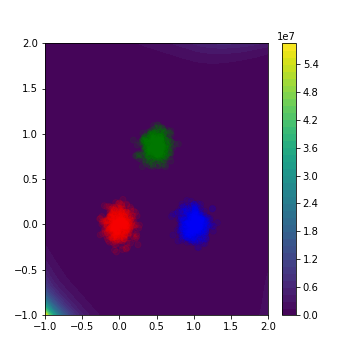
\includegraphics[width=\linewidth]{sections/010_neurips2019/paper/images/classic-narrow-alpha0.png}
        \caption{CE - $\alpha_0$}
        \label{classic-narrow-alpha0}
    \end{subfigure}
    \hspace{-0.4cm}
    \begin{subfigure}{0.26\textwidth}
        \centering
        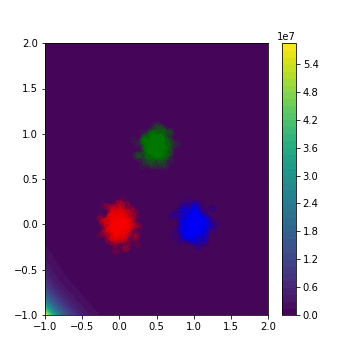
\includegraphics[width=\linewidth]{sections/010_neurips2019/paper/images/classic-narrow-alpha1.png}
        \caption{CE - $\alpha_1$}
        \label{classic-narrow-alpha1}
    \end{subfigure}
    \hspace{-0.4cm}
    \begin{subfigure}{0.26\textwidth}
        \centering
        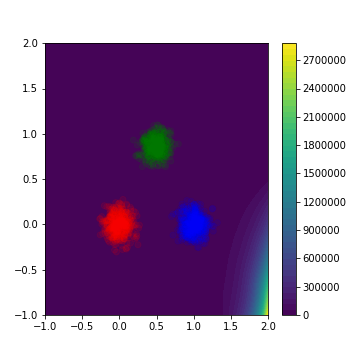
\includegraphics[width=\linewidth]{sections/010_neurips2019/paper/images/classic-narrow-alpha2.png}
        \caption{CE - $\alpha_2$}
        \label{classic-narrow-alpha2}
    \end{subfigure}
    \hspace{-0.4cm}
    \begin{subfigure}{0.26\textwidth}
        \centering
        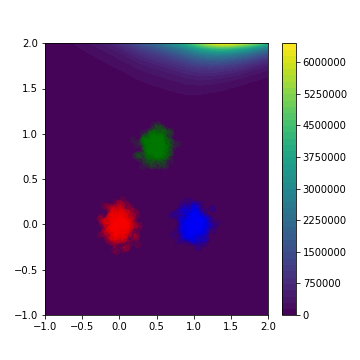
\includegraphics[width=\linewidth]{sections/010_neurips2019/paper/images/classic-narrow-alpha3.png}
        \caption{CE - $\alpha_3$}
        \label{classic-narrow-alpha3}
    \end{subfigure}

    \begin{subfigure}{0.26\textwidth}
        \centering
        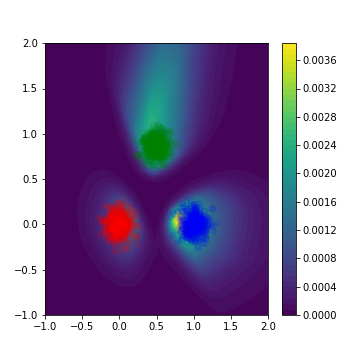
\includegraphics[width=\linewidth]{sections/010_neurips2019/paper/images/new-narrow-alpha0.png}
        \caption{UCE - $\alpha_0$}
        \label{new-narrow-alpha0}
    \end{subfigure}
    \hspace{-0.4cm}
    \begin{subfigure}{0.26\textwidth}
        \centering
        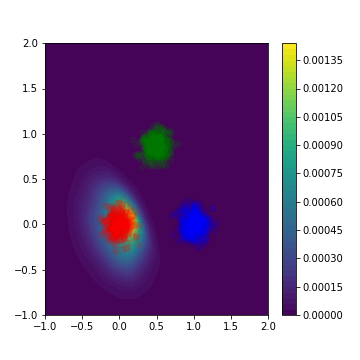
\includegraphics[width=\linewidth]{sections/010_neurips2019/paper/images/new-narrow-alpha1.png}
        \caption{UCE - $\alpha_1$}
        \label{new-narrow-alpha1}
    \end{subfigure}
    \hspace{-0.4cm}
    \begin{subfigure}{0.26\textwidth}
        \centering
        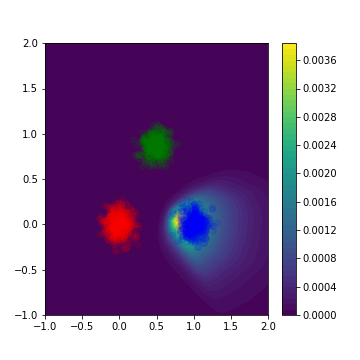
\includegraphics[width=\linewidth]{sections/010_neurips2019/paper/images/new-narrow-alpha2.png}
        \caption{UCE - $\alpha_2$}
        \label{new-narrow-alpha2}
    \end{subfigure}
    \hspace{-0.4cm}
    \begin{subfigure}{0.26\textwidth}
        \centering
        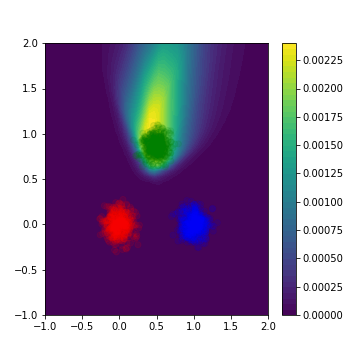
\includegraphics[width=\linewidth]{sections/010_neurips2019/paper/images/new-narrow-alpha3.png}
        \caption{UCE - $\alpha_3$}
        \label{new-narrow-alpha3}
    \end{subfigure}
    \caption{Concentration parameters of the Dirichlet distribution on a classification task with three non-overlapping Gaussians. The figures \ref{classic-narrow-alpha0}, \ref{classic-narrow-alpha1}, \ref{classic-narrow-alpha2}, \ref{classic-narrow-alpha3} are $\alpha_0$, $\alpha_1$, $\alpha_2$, $\alpha_3$ learned with the classic cross-entropy. The figures \ref{classic-narrow-alpha0}, \ref{classic-narrow-alpha1}, \ref{classic-narrow-alpha2}, \ref{classic-narrow-alpha3} are $\alpha_0$, $\alpha_1$, $\alpha_2$, $\alpha_3$ learned with the \UncertaintyLoss.}
    \label{fig:alpha_classification}
\end{figure}

\begin{figure}[H]
\centering
    \begin{subfigure}{0.26\textwidth}
        \centering
        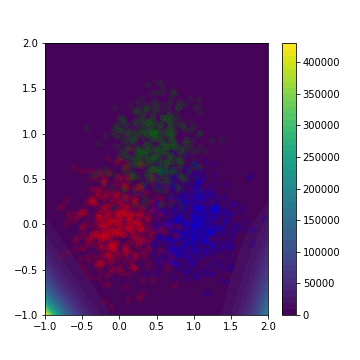
\includegraphics[width=\linewidth]{sections/010_neurips2019/paper/images/classic-spread-alpha0.png}
        \caption{CE - $\alpha_0$}
        \label{classic-spread-alpha0}
    \end{subfigure}
    \hspace{-0.4cm}
    \begin{subfigure}{0.26\textwidth}
        \centering
        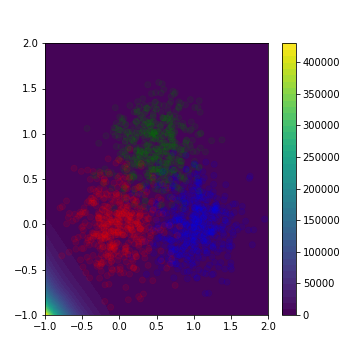
\includegraphics[width=\linewidth]{sections/010_neurips2019/paper/images/classic-spread-alpha1.png}
        \caption{CE - $\alpha_1$}
        \label{classic-spread-alpha1}
    \end{subfigure}
    \hspace{-0.4cm}
    \begin{subfigure}{0.26\textwidth}
        \centering
        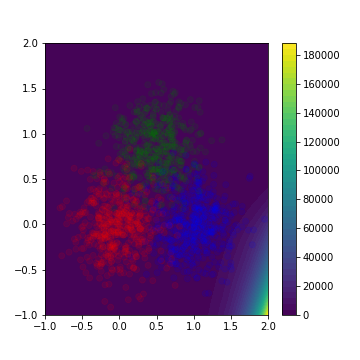
\includegraphics[width=\linewidth]{sections/010_neurips2019/paper/images/classic-spread-alpha2.png}
        \caption{CE - $\alpha_2$}
        \label{classic-spread-alpha2}
    \end{subfigure}
    \hspace{-0.4cm}
    \begin{subfigure}{0.26\textwidth}
        \centering
        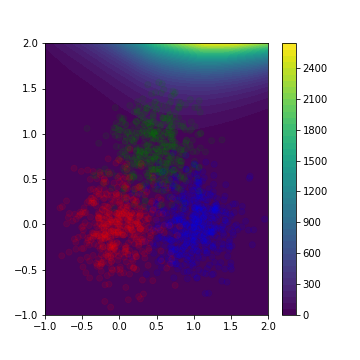
\includegraphics[width=\linewidth]{sections/010_neurips2019/paper/images/classic-spread-alpha3.png}
        \caption{CE - $\alpha_3$}
        \label{classic-spread-alpha3}
    \end{subfigure}

    \begin{subfigure}{0.26\textwidth}
        \centering
        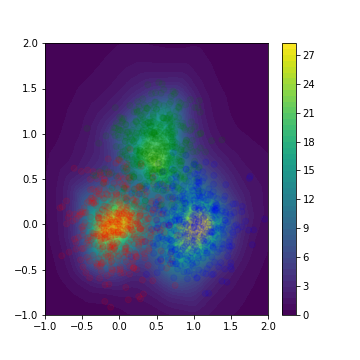
\includegraphics[width=\linewidth]{sections/010_neurips2019/paper/images/new-spread-alpha0.png}
        \caption{UCE - $\alpha_0$}
        \label{new-spread-alpha0}
    \end{subfigure}
    \hspace{-0.4cm}
    \begin{subfigure}{0.26\textwidth}
        \centering
        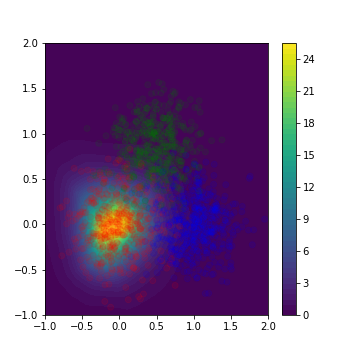
\includegraphics[width=\linewidth]{sections/010_neurips2019/paper/images/new-spread-alpha1.png}
        \caption{UCE - $\alpha_1$}
        \label{new-spread-alpha1}
    \end{subfigure}
    \hspace{-0.4cm}
    \begin{subfigure}{0.26\textwidth}
        \centering
        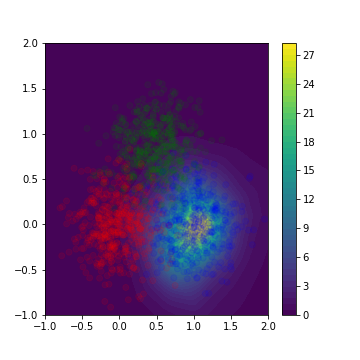
\includegraphics[width=\linewidth]{sections/010_neurips2019/paper/images/new-spread-alpha2.png}
        \caption{UCE - $\alpha_2$}
        \label{new-spread-alpha2}
    \end{subfigure}
    \hspace{-0.4cm}
    \begin{subfigure}{0.26\textwidth}
        \centering
        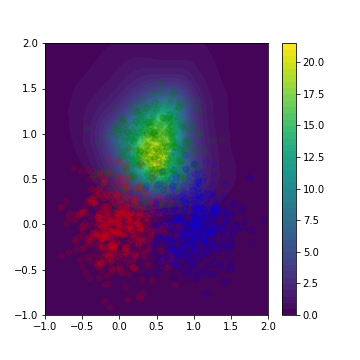
\includegraphics[width=\linewidth]{sections/010_neurips2019/paper/images/new-spread-alpha3.png}
        \caption{UCE - $\alpha_3$}
        \label{new-spread-alpha3}
    \end{subfigure}
    \caption{Concentration parameters of the Dirichlet distribution on a classification task with three non-overlapping Gaussians. The figures \ref{classic-spread-alpha0}, \ref{classic-spread-alpha1}, \ref{classic-narrow-alpha2}, \ref{classic-spread-alpha3} are $\alpha_0$, $\alpha_1$, $\alpha_2$, $\alpha_3$ learned with the classic cross-entropy. The figures \ref{classic-spread-alpha0}, \ref{classic-spread-alpha1}, \ref{classic-narrow-alpha2}, \ref{classic-spread-alpha3} are $\alpha_0$, $\alpha_1$, $\alpha_2$, $\alpha_3$ learned with the \UncertaintyLoss.}
    \label{fig:alpha_classification2}
\end{figure}

\subsection{Asynchronous Event Prediction}

In this section, we consider temporal data. The goal of this experiment is again to show the benefit of the \UncertaintyLoss compared to the classical cross-entropy in the case of asynchronous event prediction.

\textit{Set-up.} For this purpose, we use the same set-up describe in the experiment Anomaly detection \& Uncertainty. We trained the model \DirModel with three different type of losses: (1) The classical cross-entropy (CE), (2) The classical cross-entropy with regularization described in section \ref{uncertainty_loss} (CE + reg) and (3) The classical \UncertaintyLoss with regularization described in section \ref{uncertainty_loss} (UCE + reg).

\begin{figure}[H]
\centering
    \begin{subfigure}{0.3\textwidth}
        \centering
        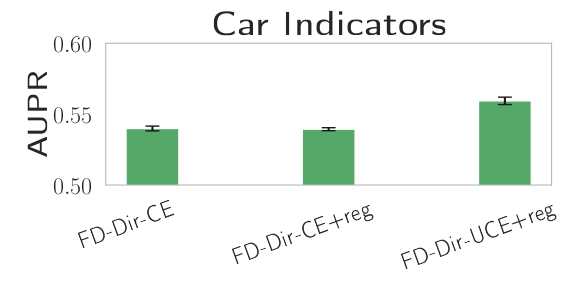
\includegraphics[width=\linewidth]{sections/010_neurips2019/paper/images/uncertainty-apr-bmw-indicator-ok3.png}
    \end{subfigure}%
    \begin{subfigure}{0.3\textwidth}
        \centering
        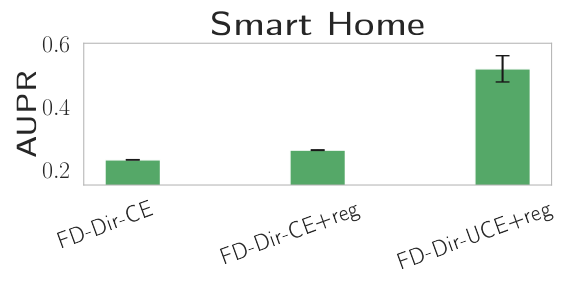
\includegraphics[width=\linewidth]{sections/010_neurips2019/paper/images/uncertainty-apr-kast-home-ok3.png}
    \end{subfigure}%
    \caption{Loss comparison in anomaly detection}
    \label{fig:loss_comparison}
    \vspace{-0.5cm}
\end{figure}

\textit{Results.} The results are shown in Fig. \ref{fig:loss_comparison}. The loss UCE + reg consistently improves the anomaly detection based on the distribution uncertainty.
